\section{Diseño}

El diseño del sistema desarrollado ha sido clave para garantizar la viabilidad técnica, la modularidad de los componentes y una experiencia de usuario intuitiva. En este apartado se describen los principales aspectos del diseño arquitectónico, conceptual y de interfaz de la solución implementada, incluyendo tanto el funcionamiento interno de los módulos como su interacción con el usuario final.

\subsection{Diseño de la arquitectura}

El sistema se integra en la plataforma Java Multimedia Retrieval (JMR), ampliando sus capacidades de búsqueda visual mediante la incorporación de un módulo generativo desarrollado en Python. La arquitectura sigue un enfoque modular y desacoplado, en el que los componentes desarrollados en Python se comunican con JMR a través de una API REST.

\begin{itemize}
    \item \textbf{Interfaz de usuario (JMR):} permite introducir descripciones textuales como entrada para la generación de consultas visuales.
    
    \item \textbf{Módulo generativo (Python):} expone una API REST que recibe descripciones textuales y devuelve imágenes generadas mediante modelos de difusión. Este módulo está encapsulado en una aplicación ligera desplegable de forma independiente.
    
    \item \textbf{Módulo de integración (Java):} dentro de JMR, se encarga de enviar peticiones HTTP a la API generativa, recuperar la imagen resultante y tratarla como una consulta visual.
    
    \item \textbf{Módulo CBIR (JMR):} compara la imagen generada con una base de datos de imágenes mediante descriptores visuales y métricas de similitud.
\end{itemize}

\begin{figure}[H]
    \centering
    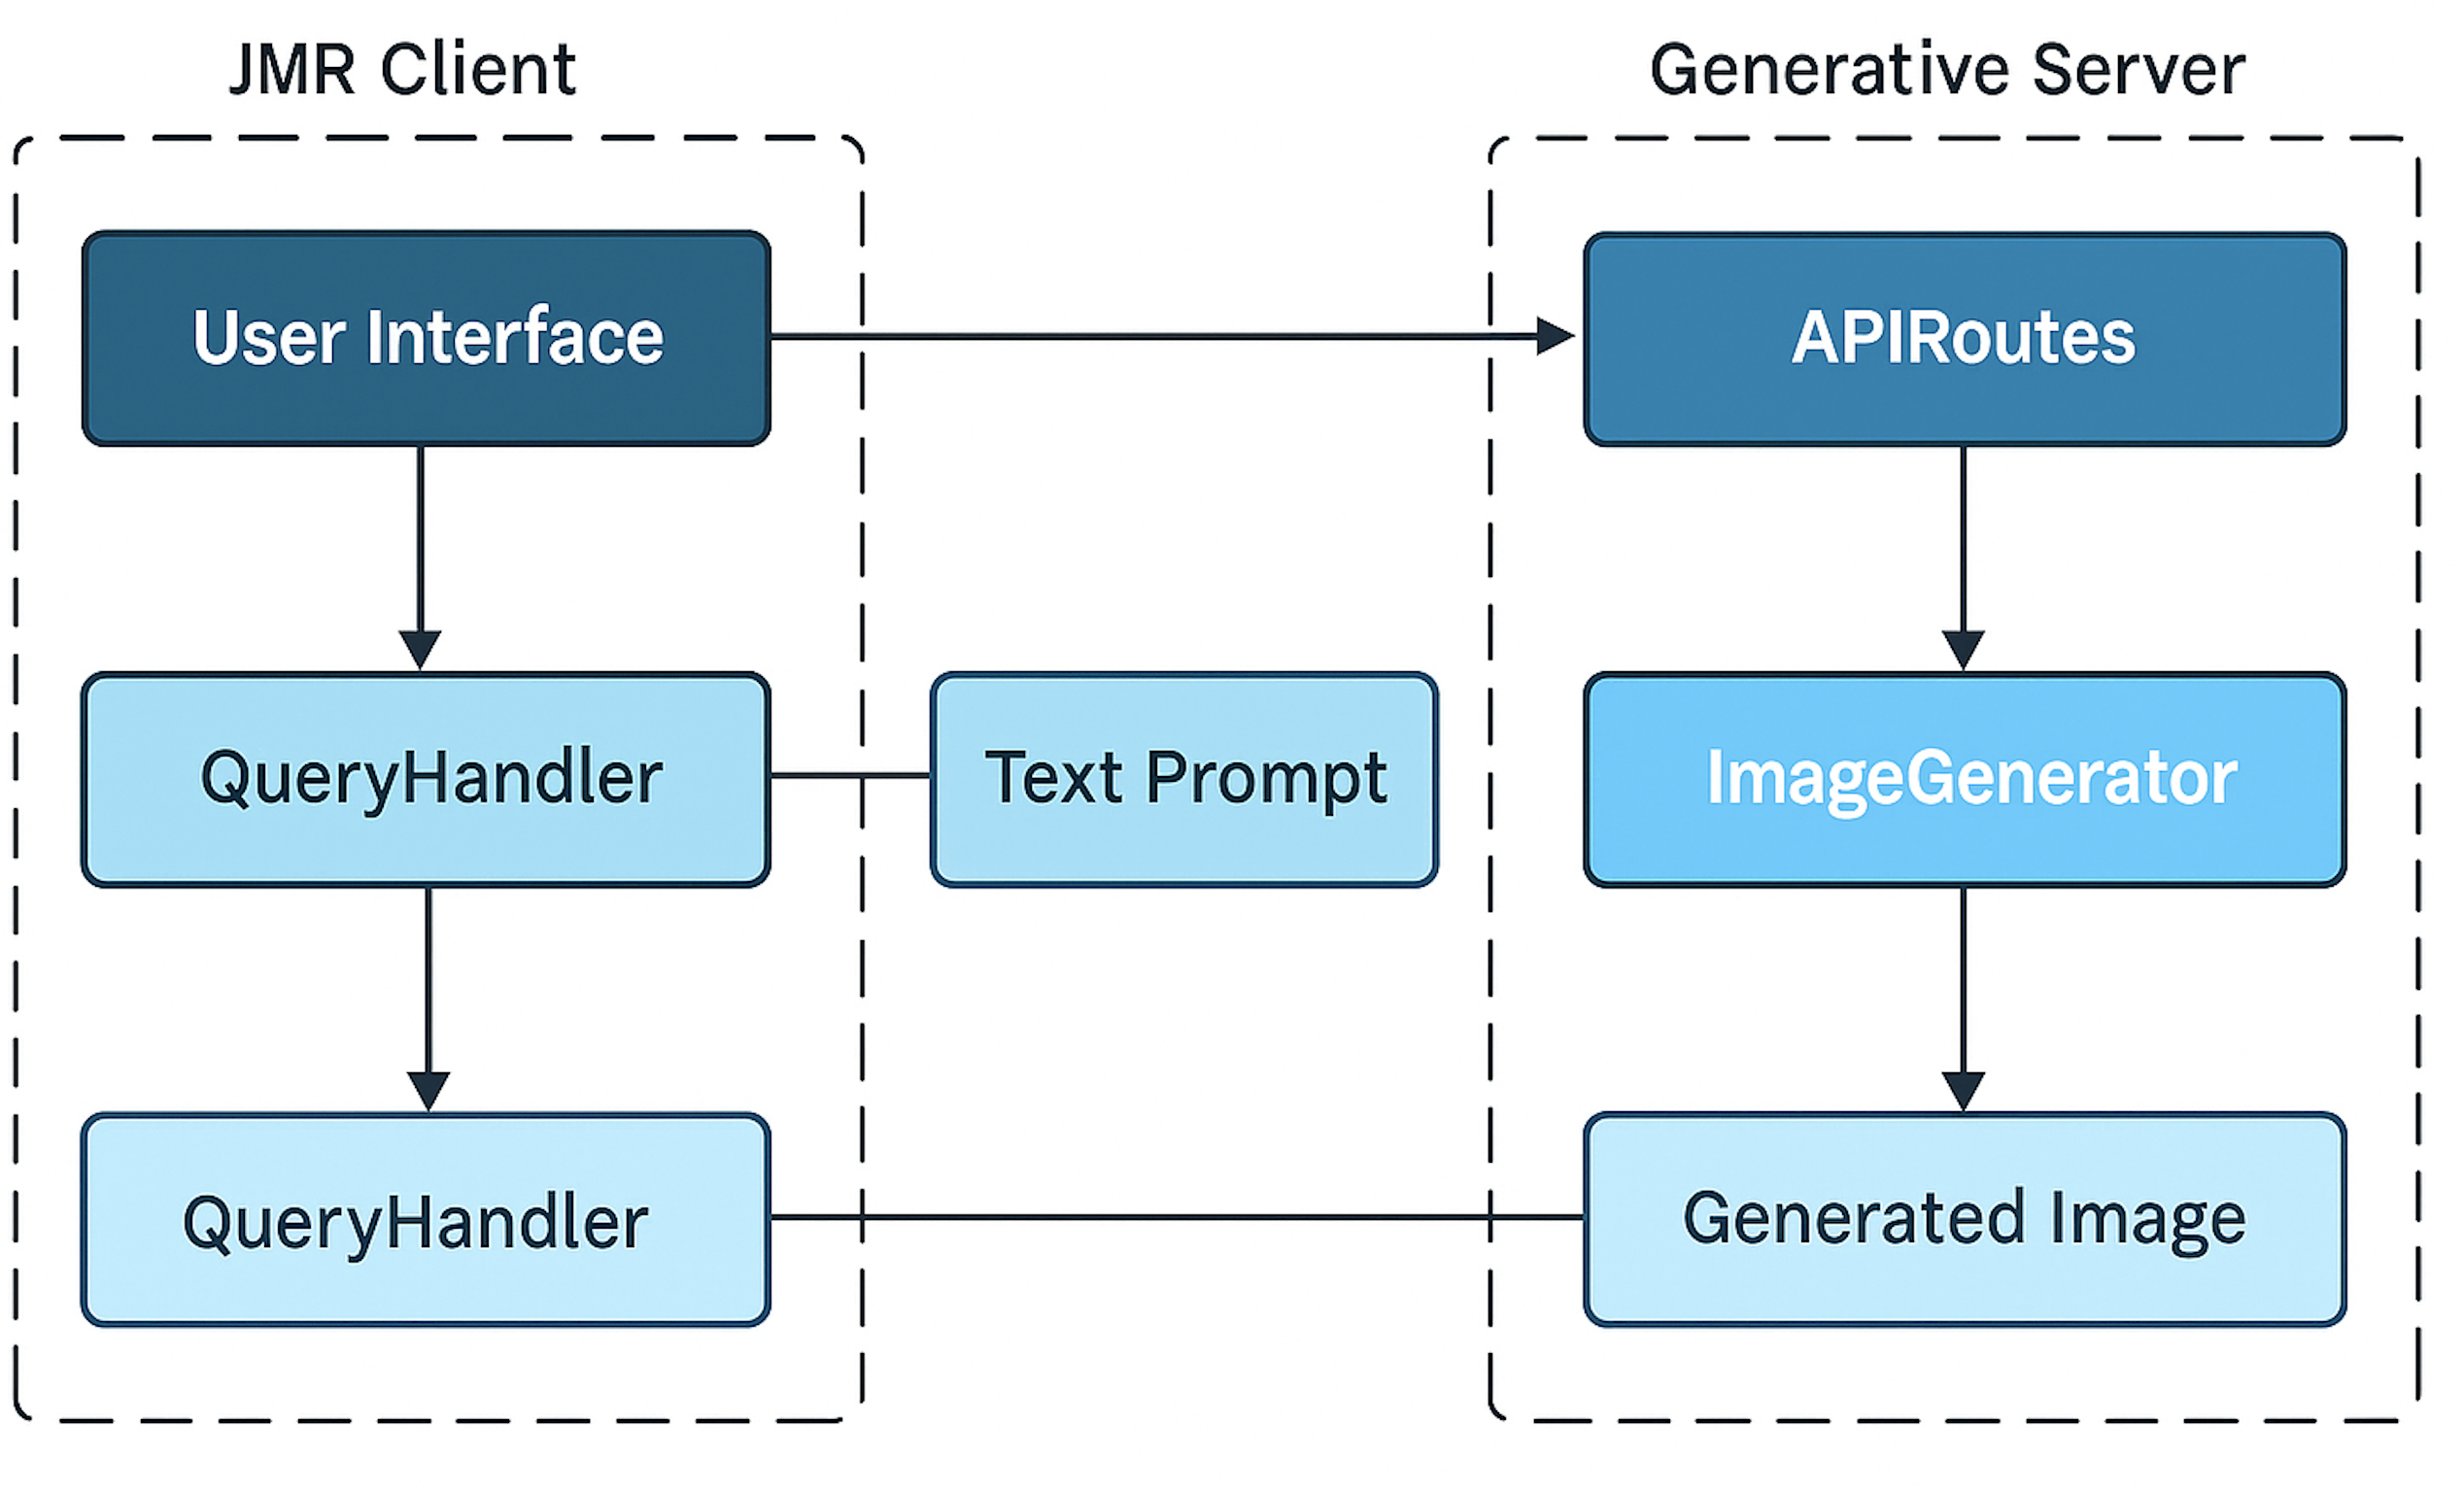
\includegraphics[width=0.7\textwidth]{nueva_arquitectura}
    \caption{Arquitectura lógica del sistema integrado}
    \label{fig:arquitectura-final}
\end{figure}

Esta arquitectura distribuida permite mejorar la mantenibilidad, facilitar la evolución del modelo generativo y adaptar el sistema a diferentes entornos sin afectar a la aplicación principal.

\subsection{Modelo conceptual}

El modelo conceptual del sistema refleja los elementos fundamentales que intervienen en el proceso de generación y búsqueda visual:

\begin{itemize}
    \item \textbf{Usuario:} introduce una descripción textual a través de la interfaz JMR.
    \item \textbf{Prompt o descripción textual:} entrada en lenguaje natural que sirve como semilla para la generación de una imagen.
    \item \textbf{Imagen generada:} salida del modelo de IA a partir del prompt introducido por el usuario.
    \item \textbf{Resultado de búsqueda:} conjunto de imágenes similares recuperadas por el motor CBIR.
    \item \textbf{Configuración del modelo:} conjunto de parámetros que determinan el comportamiento del generador (modelo base, pasos, guidance, etc.).
\end{itemize}

Este modelo permitió definir los flujos de información, el diseño de las peticiones API y las entidades clave del sistema.

\subsection{Diseño del modelo de clases}

Dado que el sistema combina componentes en dos lenguajes distintos, se ha documentado por separado el modelo de clases tanto del cliente Java como del servidor Python.

\subsubsection{Modelo de clases en Java}

El cliente JMR incluye una serie de clases que gestionan la visualización, el flujo de entrada/salida y la integración con el servidor generativo. El siguiente diagrama resume las principales clases y sus relaciones:

\begin{figure}[H]
    \centering
    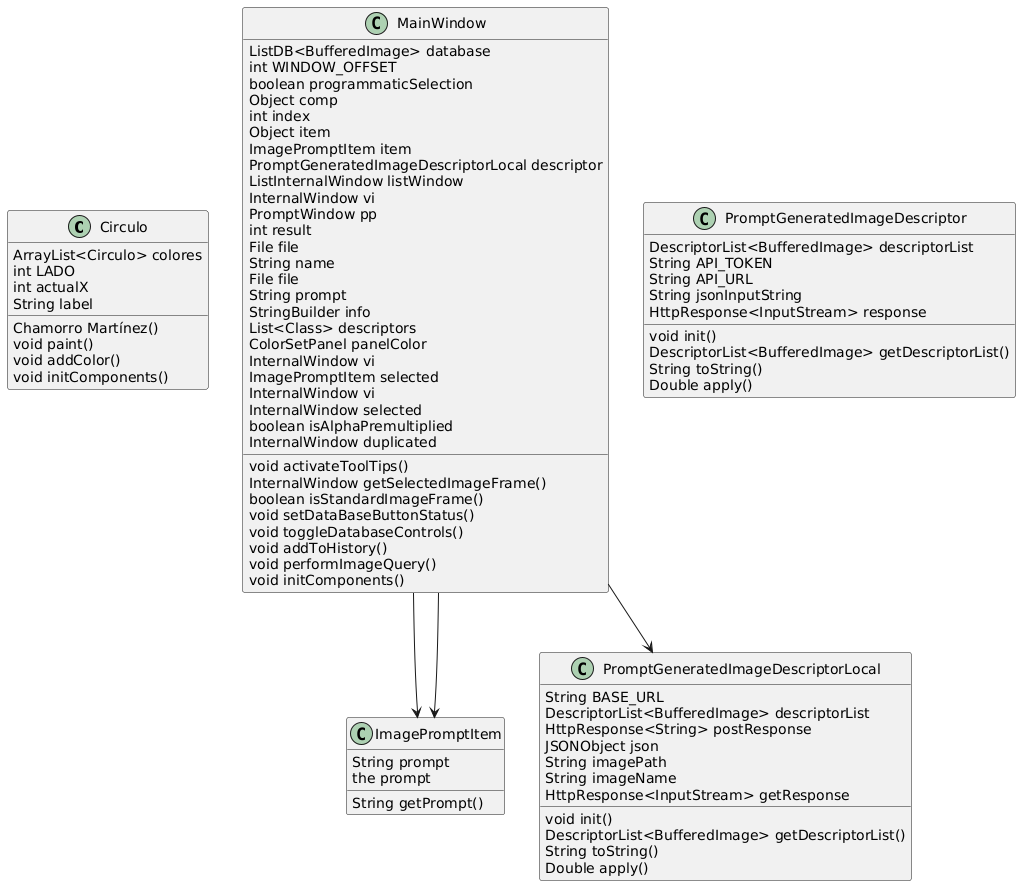
\includegraphics[width=0.85\textwidth]{diagrama_clases_java}
    \caption{Diagrama de clases del módulo de integración en Java}
    \label{fig:clases-java}
\end{figure}

\subsubsection{Modelo de clases en Python}

Aunque muchos módulos Python siguen una estructura funcional, se han representado como clases sintéticas para reflejar su cohesión interna y responsabilidades. Además, el script de entrenamiento se encapsula conceptualmente como una clase \texttt{DogTrainer}, facilitando su comprensión y documentación:

\begin{figure}[H]
    \centering
    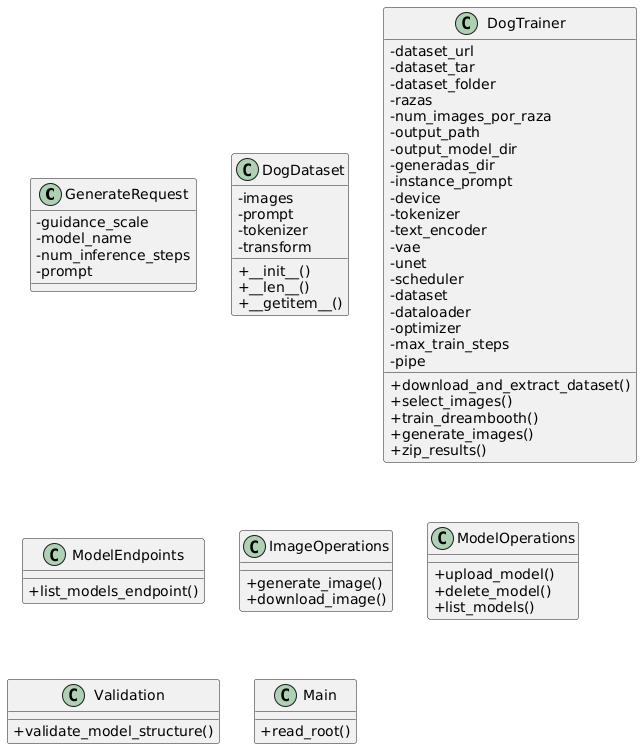
\includegraphics[width=0.85\textwidth]{diagrama_clases_python}
    \caption{Diagrama de clases del sistema generativo en Python}
    \label{fig:clases-python}
\end{figure}

Estas representaciones permiten comprender de forma estructurada la distribución de responsabilidades y la lógica interna de cada componente, sirviendo de soporte a la implementación modular del sistema.


\subsection{Diseño de la interfaz}
\subsubsection{Bocetos}
\subsubsection{Diagrama de flujo}
El siguiente diagrama de flujo describe la secuencia de operaciones que se ejecutan desde la entrada del prompt por parte del usuario hasta la recuperación de resultados visuales. Este flujo ilustra la lógica general del sistema y su ejecución coordinada entre los distintos módulos.

\begin{figure}[H]
    \centering
    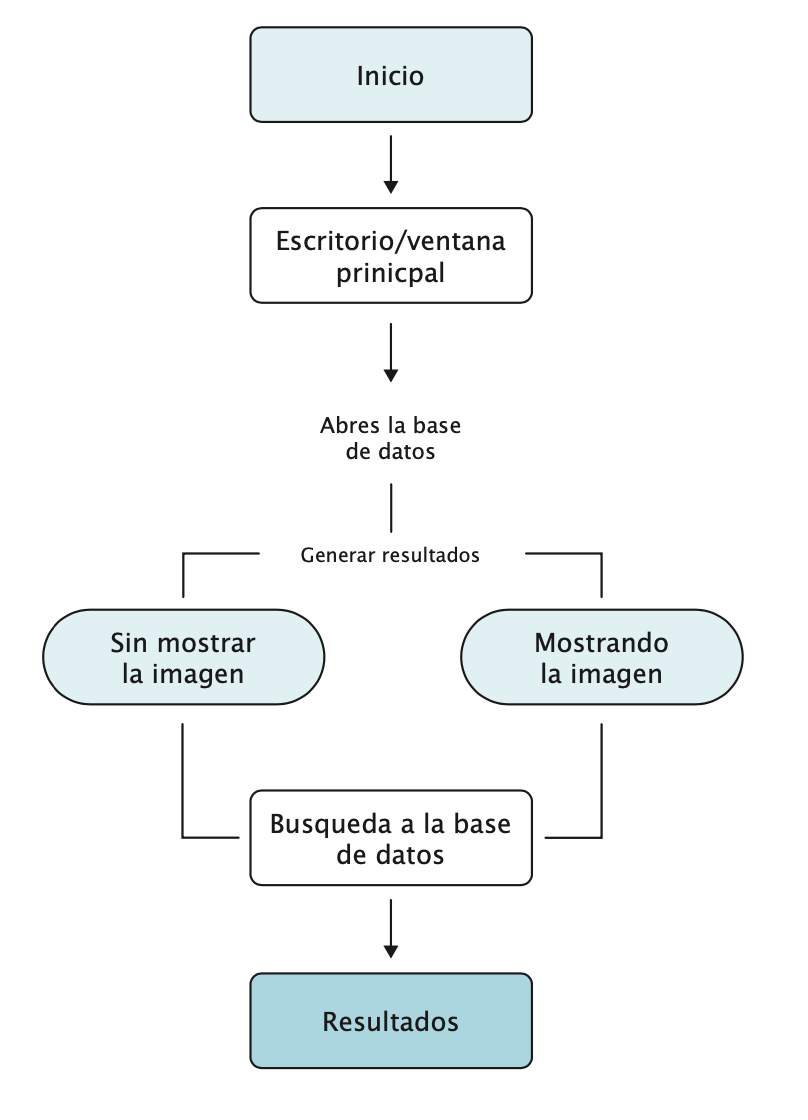
\includegraphics[width=0.8\textwidth]{diagrama_flujo}
    \caption{Flujo de interacción entre el usuario, la API generativa y el sistema CBIR}
    \label{fig:flujo-interaccion}
\end{figure}

\subsubsection{Usabilidad}
El diseño del sistema ha sido guiado por criterios de usabilidad orientados a garantizar una interacción clara, eficiente y accesible para usuarios con distintos niveles de experiencia técnica. A partir de las historias de usuario definidas (HU1 y HU2), se identificaron las necesidades prioritarias que la interfaz debía cubrir: introducir una descripción textual de forma sencilla, obtener una imagen generada coherente con dicha descripción, y utilizar esa imagen como punto de partida para la búsqueda de contenido visual similar.

En respuesta a estos objetivos, se adoptaron los siguientes principios de diseño centrado en el usuario:
\begin{itemize}
    \item \textbf{Simplicidad de la interacción:} La interfaz principal se reduce a tres elementos fundamentales: un campo de entrada para el texto (prompt), un botón de acción para generar la imagen, y un área de visualización para mostrar el resultado. Esta estructura minimalista reduce la curva de aprendizaje y evita distracciones innecesarias.
    
    \item \textbf{Visibilidad y retroalimentación inmediata:} Una vez introducido el prompt y pulsado el botón de generación, el sistema muestra un indicador de carga que informa al usuario del progreso del proceso. Al finalizar, se muestra la imagen resultante junto con la posibilidad de confirmar su uso como consulta CBIR. Esta respuesta inmediata refuerza la confianza del usuario en el sistema.
    
    \item \textbf{Consistencia y familiaridad:} Se respetaron patrones comunes de interacción para minimizar la necesidad de aprendizaje. El uso de botones estándar, etiquetas claras y una disposición vertical favorecen una navegación predecible y consistente.
\end{itemize}

En conjunto, estas decisiones buscan asegurar que el sistema no solo sea técnicamente funcional, sino también fácil de utilizar, confiable y accesible. El objetivo es permitir que cualquier usuario, independientemente de su formación técnica, pueda interactuar con el sistema para explorar visualmente una idea expresada mediante lenguaje natural.
